\section{Overview}
The application of mathematics has played a key role in the development of technological advancements and breakthroughs in sciences. Throughout history, mathematics has provided us with an increasing amount of various sub branches such as discrete maths, applied maths, cartesian geometry, algebra, calculus and many more. All of which can be applied to the real world, whether it is for construction, physics or day to day life. 

A key branch under discrete mathematics is graph theory where models can be developed that represents relationships between different objects. Graphs has a range of uses both in the mathematical world and the real world. They can be used to visually represent large sets of numerical data so that different properties can be derived from the graph such as clustering of certain areas, the connectivity between vertices or edges and the correlations that they may have. They are also widely known as networks with some examples such as a friendship network, business networks and even a food chain levels. These are the areas that I will explore along with a way to visualise them by using python. Analysing specific properties that may influence the visualisation of the graphs and thus the outcome of the relationships between the vertices.

\section{History}
Initially, graph theory was introduced in 1735 as a form of solution to the seven bridges of Königsberg problem which solved by Leonard Euler\cite{POWELL20151}. This famous problem involved an island within Königsberg that had a river, Pregel, surrounding the island via a fork, there were seven bridges that crossed this river from the island to other major landmasses of Königsberg, Prussia. The island had four bridges, two north, two south onto the mainland, one bridge to a neighbouring island and the neighbouring island itself had two bridges which totals to the seven bridges stated by the problem, see Figure \ref{fig:Königsberg's Bridges}. 

Due to the location in which the island was situated, the problem was to determine whether a route exists that manoeuvres through all the bridges exactly once and must return to the starting location. Leonard Euler proceeded to analyse the problem by evaluating the only the key areas, this was the land masses and the bridges. Other information such as the sizes of the island, bridge type or length were irrelevant. Consequently, the problem could be portrayed via dots and lines to give a simplistic view (Figure \ref{fig:Königsberg's Graph}), once developed, this was known as vertices which denoted the key interest and the edges that are incident to the vertices to denote the connections/relations between them. 

By removing the irrelevant information, Euler was able to simplify and visualise the problem thus discovering the fact that for there to be a solution, each vertex must have an even number of edges incident to the vertex (even degree) as you require one edge for entering and another for exiting otherwise not all edges will be part of the final path. All vertices in the Königsberg problem have odd degree, thus what's known as an \emph{Eulerian path} (a path that traverses all edges exactly once) doesn't exist for this problem and since a Eulerian path doesn't exist then a \emph{Eulerian circuit} cannot exist either (a Eulerian path that returns to the starting vertex). Therefore Euler's solution proves that there is no solution to the seven bridges of Königsberg and is regarded as the first proof in relation to graphs. This led to the birth of graph theory.

\begin{figure}[!htb]
\centering
\begin{subfigure}{.45\textwidth}
	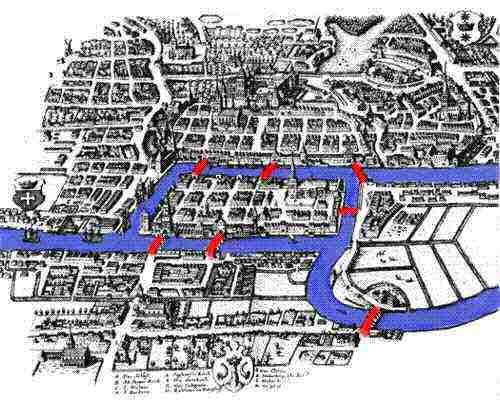
\includegraphics[scale=0.4]{Konigsberg}
	\caption{Königsberg and the seven bridges, from MacTutor Archive \cite{MacTutor}}
	\label{fig:Königsberg's Bridges}
\end{subfigure}
\hfill
\begin{subfigure}{.45\textwidth}
	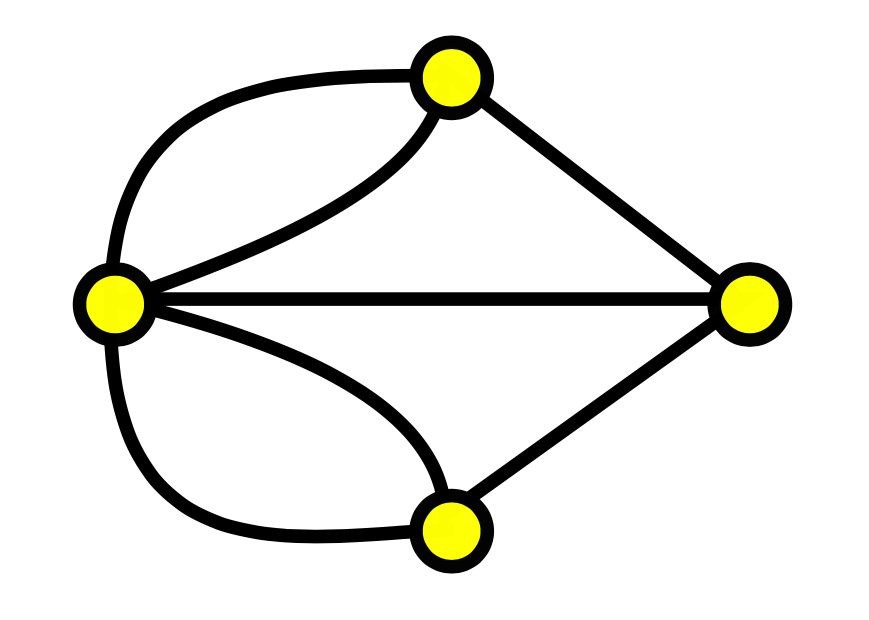
\includegraphics[scale=0.2]{Konigsgraph}
	\caption{Graph representation to Königsberg problem from online source \cite{Katie}}
	\label{fig:Königsberg's Graph}
\end{subfigure}
\caption{The original seven bridges of Königsberg and it's graph representation that only focusses on the key details and disregards the irrelevant information. Achieved by the use of vertices and edges.}
\end{figure}

After Eulerian paths and cycles were introduced, the next famous puzzle in relation to graph theory was invented in 1857 and was known as the Icosian Game\cite{carlson_2022} by William Rowan Hamilton. The objective of the puzzle was to find a cycle that visits all vertices exactly once and returns to the starting vertex. This type of cycle is later called a \emph{Hamilton cycle} along with the definition of a \emph{Hamilton path} which doesn't have the requirement to return to the starting vertex.

In the mathematical world, Leonard Euler is known for the \emph{Euler's identity} within complex mathematics which states that for a real number $x$, $e^{ix}=\cos(x)+i\sin(x)$. This has been crucial in many subject areas such as in physics and engineering. Additionally, in 1850, Euler uncovered another formula to be known as \emph{Euler's polyhedra formula} which states that $F + V - E = 2$ where $F$ denotes the number of faces, $V$ as the number of vertices and the number of edges as $E$ of this graph model. As polyhedrons can be depicted as graphs, algebraic topology benefited from Euler's polyhedron formula where more complex surfaces could be studied such as the surface of a torus. Based upon this formula, the \emph{Euler characteristic} was formalised to describe the topological characteristic of various complex surfaces with it's formula as $F + V - E = 2 - 2g$ where $g$ is denotes the number of "holes" the surface has (formally known as the genus). 

Furthermore, graph theory has assisted in problems such as the four-colour map problem in the 1850s that states whether all the countries can be coloured with only four colours on a map such that no adjacent countries were coloured with the same colour. In which the solution wasn't found until 1972 by Kenneth Appel and Wolfgang Haken\cite{Ohnishi2009} through the assistance of a computer. An example of a four colour problem is colouring the counties in the UK with only four colours and the solution for this is shown in Figure \ref{fig:UK 4 colour}.
\newline

\begin{figure}[!htb]
\centering
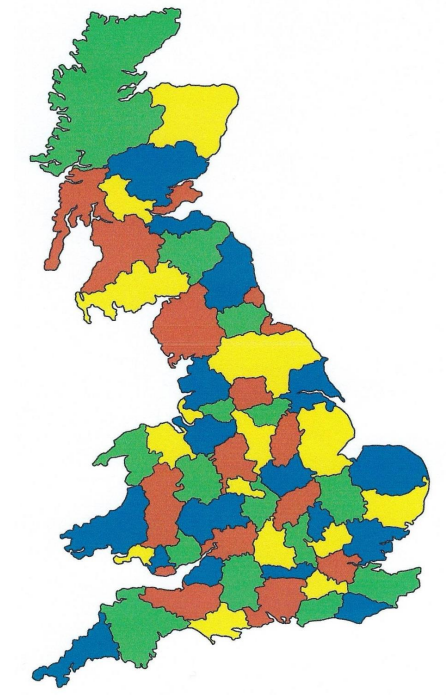
\includegraphics[scale=0.45]{4colourUK}
\caption{The solution for the four colour map problem with regards to the counties in the UK sourced from Robin Wilson \cite{4ColourRobin}.}
\label{fig:UK 4 colour}
\end{figure}

The Chinese postman problem is another such graph theory problem where you must find the shortest path that uses all the edges in the graph at least once. A similar alternate version is called the travelling salesman problem where you find a shortest path that uses all edges exactly once in the graph and must end at the starting vertex. These such problems are used in Linear programming to find optimal solution in routing or pathing between locations. Variants of the CPP (Chinese postman problem) includes undirected Chinese postman problem (UCPP) which contains different restrictions depending on the subset of edges (see the paper \cite{IrnichStefan2008Uppw}) and Chinese Postman Problem with load-dependent costs (CPP-LC\cite{CorberánÁngel2018TCPP}) that includes weights upon the edges so that an optimal route can be generated. This can be widely used and applied to problems such as the best route to lower vehicle CO$_2$ emissions. So these problems can be applied to the modern day scenarios and are still valuable to companies now.
\newline

Therefore graph theory studies have been researched extensively since 1735 with many beneficial factors brought into the real world. This is possible due to the versatile nature that data structures in the real world can be represented as a mathematical structure as graphs/networks. Examples of what they can represent ranges from simple relationships between people to the complex structure of the brain by studying it's anatomic structure and assigning vertices according to the sections of the brains and edges as the links between them. The links are typically representations of the neurons in the brain. Further detail of brain mapping into graphs can be read by the paper \cite{articlebrain}. Therefore by using graph models, various patterns and correlations can then be derived to generate graph properties that can be studied to develop useful information and possible improvements to the whole graph.

\section{Basic notation and terminology}
Graphs or networks are mathematical constructs that are formed by a collection of vertices and edges. Vertices $V$ represents individual objects such as land masses, companies, houses, people etc. Edges $E$ represents the connections between the vertices such as their relationship, flow of water, supply chain etc. Sets $V(G)$ or $V$ and $E(G)$ or $E$ forms the graph $G$ and can be written as $G=(V, E)$ with E being a subset of $V \times V$ so an edge $e \in E$ can be written as $v_{1}v_{2}$ if $e$ connects $v_{1}$ and $v_{2}$ where $v_{1}, v_{2} \in V$. There's variation among the graphs as they can be directed or undirected, the edges may carry weights and they may contain self loops. Figure \ref{fig:Simple Graph} and \ref{fig:Directed Graph} shows simple graphs, one of which is undirected and another which is directed. A graph $H = (V', E')$ is a \emph{subgraph} of $G=(V, E)$ if $V' \subset V$ and $E' \subset E$.

\emph{Order} is the mathematical term that represents the number of the vertices in the vertex set $V(G)$. \emph{Size} is number of vertices in the edge set $E(G)$. The \emph{degree} of a vertex, denoted by $deg(v)$ is the number of edges that are connected (otherwise known as \emph{incident}) to the vertex, discussed previously in Euler's solution to the seven bridges of Königsberg problem. Additionally, $\delta(G)$ and $\Delta(G)$ represents the minimum and maximum degree in $G$ respectively. $G$ is a \emph{regular} graph if $\delta(G) = \Delta(G)$. Vertices $v_{1}$ and $v_{2}$ are \emph{adjacent} if there exists an edge $e \in E$ that connects them. Vertex $v_{2}$ is also known as a \emph{neighbour} to $v_{1}$ and is part of the set $N(v_{1})$ which denotes the neighbours of $v_{1}$. 
\newline

\begin{figure}[!htb]
\centering
\begin{subfigure}{.45\textwidth}
	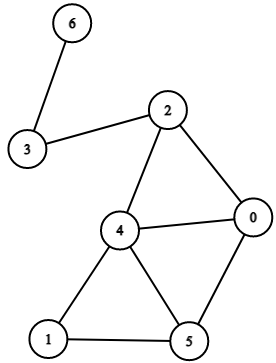
\includegraphics[scale=0.8]{simplegraph}
	\caption{An undirected graph with 7 vertices, 9 edges and a average vertex degree of $18/7$}
	\label{fig:Simple Graph}
\end{subfigure}
\hfill
\begin{subfigure}{.45\textwidth}
	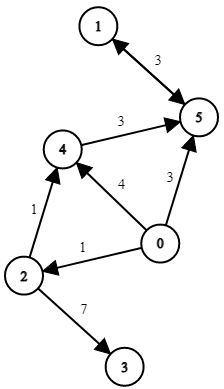
\includegraphics[scale=0.8]{directedgraph}
	\caption{A directed graph with 7 vertices and 7 directed edges that contain weights}
	\label{fig:Directed Graph}
\end{subfigure}
\caption{The 2 simple types of graphs within graph theory that are the basic building blocks for more complex structures and theorems.}
\end{figure}

There are multiple ways to traverse a graph. A \emph{walk} $w = v_1v_2v_3v_4v_5...v_n$ is a sequence of vertices such that $E(w) = (v_1v_2,...,v_{n-1}v_n)$ where vertices and edges can be repeated. They can be \emph{open} or \emph{closed} depending if the final vertex is equal to the starting vertex. A \emph{trail} is an open walk where no edges are repeated but vertices may be repeated. When all the edges are traversed exactly once, it's known as a \emph{Eulerian trail} (mentioned previously as a Eulerian path) and the graph is called \emph{semi-eulerian} or \emph{traversable}. Similarly for a trail that's closed (returns to the start), then it is known as a \emph{circuit} and if all edges are used then it's called a \emph{Eulerian circuit} (or Eulerian cycle) and the graph is defined to be \emph{Eulerian}. A \emph{path} is a trail but with no vertex repetitions and if the size of the path is equal to the size of the graph then it's a \emph{Hamilton path}. Finally, a \emph{cycle} is a path that ends at the starting vertex and if all vertices are visited exactly once then it's known as a \emph{Hamilton cycle} meaning that the graph is \emph{Hamiltonian}.
\newline

When considering network with flows, vertices can be known as nodes and may have capacities that limit the overall flow through the network shown in Figure \ref{fig:Network Flow}. These networks are especially used when considering plumbing, water pipes and even evacuation routes in a building. Within a room there's a capacity that is represented by it's node capacity and the weights of the edges can demonstrate the rate of flow along with it's maximal flow, i.e. when people are evacuating a building, the corridors have a limit to the amount of people that may pass through. Networks can be used to model social network processes through the study of small corporate groups to generate a communications network. This network representation will have a flow of sentiments based on social network theory\cite{ZACHARY1984259} that is constrained in three ways. Firstly by any existing direct relationships within the group, that will be denoted by vertices. Secondly, the frequency of communication of the relationships defined in the first point. Lastly, the breadth of the existing relationships in the network. Thus, by using graphs and networks, social behaviours with groups or companies can be studied on giving ways to more phycological information through numerical data.
\newline

\begin{figure}[!htb]
\centering
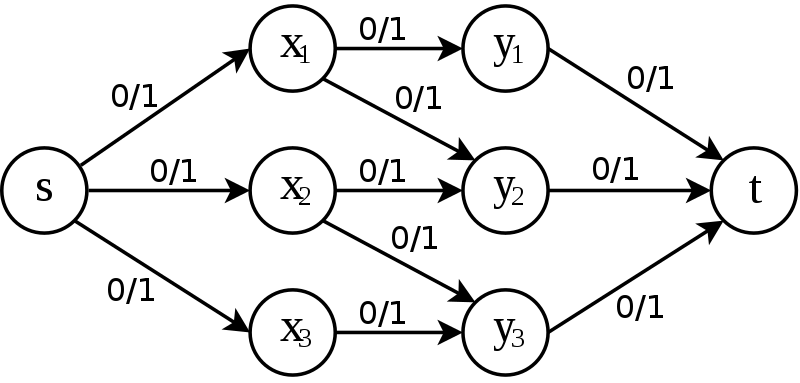
\includegraphics[scale=0.4]{networkflow}
\caption{A simple network flow with a source node and a sink node, the current flow is 0 and the edge capacities are shown. The image is sourced from Wikipedia \cite{wikinetwork}.}
\label{fig:Network Flow}
\end{figure}

Additionally they can be represented by the use of matrices to enable the use of matrix calculations on the data sets. They're known as \emph{adjacency matrices}\cite{KnauerU.2011Agt:} and within this matrix holds the number of edges incident to each vertex and it's connection based on the location of this value as the rows and columns represents the vertices. A \emph{weighted adjacency matrix} will instead hold the weights of each edge in the matrix. An $n \times n$ adjacency matrix $A = (a_{ij})$ for $ i, j = 1, ..., n$ is defined by $a_{ij} = 1$ if there exists an edge from vertex $i$ to vertex $j$. A matrix is always symmetric when considering an undirected simple graph as an edge will contribute to both sides of the matrix. Examples of an adjacency matrix along with it's graph representation is shown in Figure \ref{fig:Adjacency Graph}.
\newline

\begin{figure}[!htb]
\centering
$\vcenter{\hbox{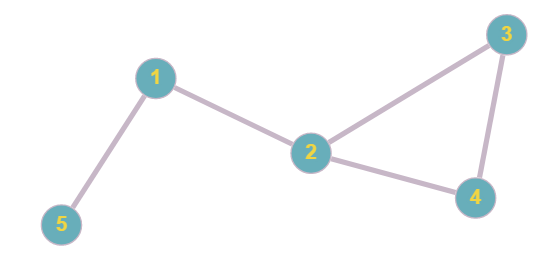
\includegraphics[scale=0.6]{adjgraph}}}$
\hfill
$A = \begin{pmatrix}
0 & 1 & 0 & 0 & 1 \\
1 & 0 & 1 & 1 & 0 \\
0 & 1 & 0 & 1 & 0 \\
0 & 1 & 1 & 0 & 0 \\
1 & 0 & 0 & 0 & 0 \\
\end{pmatrix} $
\caption{A simple graph along with it's adjacency matrix.}
\label{fig:Adjacency Graph}
\end{figure}

The main focus for future chapters will be on weighted directed graphs and the data that can be perceived by them. Chapter 2 will describe and outline specific graph properties that will be applied to datasets. This means that by analysing the graphs, numerical values can be generated to represent certain factors of the graph. These factors can then be applied to the graph to rearrange it's shape so that further correlation can be identified between all the vertices and edges.

